\documentclass{standalone}
\usepackage{tikz}
\usetikzlibrary{patterns, positioning}


\begin{document}
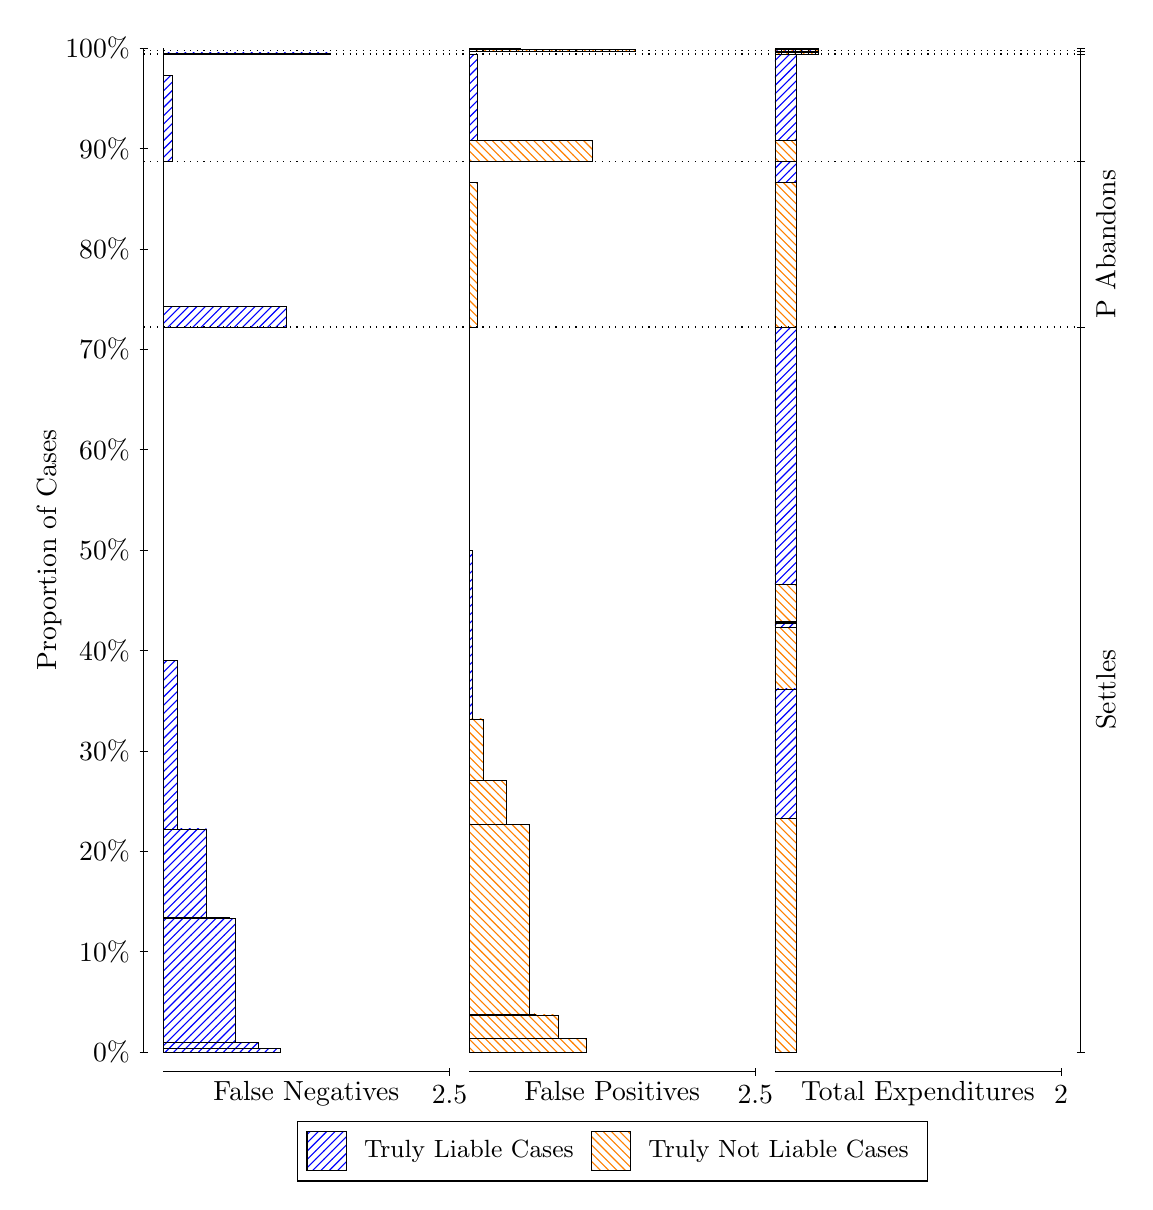
\begin{tikzpicture}
\draw[black, very thin] (1.5,1.75) -- (1.5,14.5);
\node[rotate=90, text=black, anchor=center] at (0.3, 8.125) {Proportion of Cases};
\draw[black, very thin] (1.45,1.75) -- (1.55,1.75);
\node[text=black, anchor=east] at (1.45, 1.75) {0\%};
\draw[black, very thin] (1.45,3.025) -- (1.55,3.025);
\node[text=black, anchor=east] at (1.45, 3.025) {10\%};
\draw[black, very thin] (1.45,4.3) -- (1.55,4.3);
\node[text=black, anchor=east] at (1.45, 4.3) {20\%};
\draw[black, very thin] (1.45,5.575) -- (1.55,5.575);
\node[text=black, anchor=east] at (1.45, 5.575) {30\%};
\draw[black, very thin] (1.45,6.85) -- (1.55,6.85);
\node[text=black, anchor=east] at (1.45, 6.85) {40\%};
\draw[black, very thin] (1.45,8.125) -- (1.55,8.125);
\node[text=black, anchor=east] at (1.45, 8.125) {50\%};
\draw[black, very thin] (1.45,9.4) -- (1.55,9.4);
\node[text=black, anchor=east] at (1.45, 9.4) {60\%};
\draw[black, very thin] (1.45,10.675) -- (1.55,10.675);
\node[text=black, anchor=east] at (1.45, 10.675) {70\%};
\draw[black, very thin] (1.45,11.95) -- (1.55,11.95);
\node[text=black, anchor=east] at (1.45, 11.95) {80\%};
\draw[black, very thin] (1.45,13.225) -- (1.55,13.225);
\node[text=black, anchor=east] at (1.45, 13.225) {90\%};
\draw[black, very thin] (1.45,14.5) -- (1.55,14.5);
\node[text=black, anchor=east] at (1.45, 14.5) {100\%};

\draw[black, very thin] (13.4,1.75) -- (13.4,14.5);
\draw[black, very thin] (13.35,1.75) -- (13.45,1.75);
\node[anchor=west] at (13.35, 1.75) {};
\draw[black, very thin] (13.35,10.957) -- (13.45,10.957);
\node[anchor=west] at (13.35, 10.957) {};
\draw[black, very thin] (13.35,13.058) -- (13.45,13.058);
\node[anchor=west] at (13.35, 13.058) {};
\draw[black, very thin] (13.35,14.424) -- (13.45,14.424);
\node[anchor=west] at (13.35, 14.424) {};
\draw[black, very thin] (13.35,14.464) -- (13.45,14.464);
\node[anchor=west] at (13.35, 14.464) {};
\draw[black, very thin] (13.35,14.5) -- (13.45,14.5);
\node[anchor=west] at (13.35, 14.5) {};

\draw[black, very thin, pattern color=blue, pattern=north east lines] (1.75,1.75) rectangle (3.2397,1.7987);
\draw[black, very thin, pattern color=blue, pattern=north east lines] (1.75,1.7987) rectangle (2.949,1.8747);
\draw[black, very thin, pattern color=blue, pattern=north east lines] (1.75,1.8747) rectangle (2.6583,3.4494);
\draw[black, very thin, pattern color=blue, pattern=north east lines] (1.75,3.4494) rectangle (2.5857,3.4586);
\draw[black, very thin, pattern color=blue, pattern=north east lines] (1.75,3.4586) rectangle (2.295,4.5823);
\draw[black, very thin, pattern color=blue, pattern=north east lines] (1.75,4.5823) rectangle (1.9317,6.7266);
\draw[black, very thin, pattern color=orange, pattern=north west lines] (1.75,6.7266) rectangle (1.75,10.957);
\draw[black, very thin, pattern color=blue, pattern=north east lines] (1.75,10.957) rectangle (3.3123,11.222);
\draw[black, very thin, pattern color=orange, pattern=north west lines] (1.75,11.222) rectangle (1.75,13.058);
\draw[black, very thin, pattern color=blue, pattern=north east lines] (1.75,13.058) rectangle (1.859,14.155);
\draw[black, very thin, pattern color=orange, pattern=north west lines] (1.75,14.155) rectangle (1.75,14.424);
\draw[black, very thin, pattern color=blue, pattern=north east lines] (1.75,14.424) rectangle (3.8573,14.438);
\draw[black, very thin, pattern color=orange, pattern=north west lines] (1.75,14.438) rectangle (1.75,14.464);
\draw[black, very thin, pattern color=orange, pattern=north west lines] (1.75,14.464) rectangle (1.75,14.478);
\draw[black, very thin, pattern color=blue, pattern=north east lines] (1.75,14.478) rectangle (1.75,14.5);
\draw[black, very thin, pattern color=orange, pattern=north west lines] (5.6333,1.75) rectangle (7.123,1.9256);
\draw[black, very thin, pattern color=orange, pattern=north west lines] (5.6333,1.9256) rectangle (6.7597,2.22);
\draw[black, very thin, pattern color=orange, pattern=north west lines] (5.6333,2.22) rectangle (6.469,2.2345);
\draw[black, very thin, pattern color=orange, pattern=north west lines] (5.6333,2.2345) rectangle (6.3963,4.6443);
\draw[black, very thin, pattern color=orange, pattern=north west lines] (5.6333,4.6443) rectangle (6.1057,5.1962);
\draw[black, very thin, pattern color=orange, pattern=north west lines] (5.6333,5.1962) rectangle (5.815,5.9801);
\draw[black, very thin, pattern color=blue, pattern=north east lines] (5.6333,5.9801) rectangle (5.6697,8.1243);
\draw[black, very thin, pattern color=blue, pattern=north east lines] (5.6333,8.1243) rectangle (5.6333,10.957);
\draw[black, very thin, pattern color=orange, pattern=north west lines] (5.6333,10.957) rectangle (5.7423,12.793);
\draw[black, very thin, pattern color=blue, pattern=north east lines] (5.6333,12.793) rectangle (5.6333,13.058);
\draw[black, very thin, pattern color=orange, pattern=north west lines] (5.6333,13.058) rectangle (7.1957,13.327);
\draw[black, very thin, pattern color=blue, pattern=north east lines] (5.6333,13.327) rectangle (5.7423,14.424);
\draw[black, very thin, pattern color=orange, pattern=north west lines] (5.6333,14.424) rectangle (5.6333,14.45);
\draw[black, very thin, pattern color=blue, pattern=north east lines] (5.6333,14.45) rectangle (5.6333,14.464);
\draw[black, very thin, pattern color=orange, pattern=north west lines] (5.6333,14.464) rectangle (7.7407,14.478);
\draw[black, very thin, pattern color=blue, pattern=north east lines] (5.6333,14.478) rectangle (6.2873,14.5);
\draw[black, very thin, pattern color=orange, pattern=north west lines] (9.5167,1.75) rectangle (9.7892,4.7118);
\draw[black, very thin, pattern color=blue, pattern=north east lines] (9.5167,4.7118) rectangle (9.7892,6.3625);
\draw[black, very thin, pattern color=orange, pattern=north west lines] (9.5167,6.3625) rectangle (9.7892,7.1463);
\draw[black, very thin, pattern color=blue, pattern=north east lines] (9.5167,7.1463) rectangle (9.7892,7.195);
\draw[black, very thin, pattern color=orange, pattern=north west lines] (9.5167,7.195) rectangle (9.7892,7.2094);
\draw[black, very thin, pattern color=blue, pattern=north east lines] (9.5167,7.2094) rectangle (9.7892,7.2186);
\draw[black, very thin, pattern color=orange, pattern=north west lines] (9.5167,7.2186) rectangle (9.7892,7.6886);
\draw[black, very thin, pattern color=blue, pattern=north east lines] (9.5167,7.6886) rectangle (9.7892,10.957);
\draw[black, very thin, pattern color=orange, pattern=north west lines] (9.5167,10.957) rectangle (9.7892,12.793);
\draw[black, very thin, pattern color=blue, pattern=north east lines] (9.5167,12.793) rectangle (9.7892,13.058);
\draw[black, very thin, pattern color=orange, pattern=north west lines] (9.5167,13.058) rectangle (9.7892,13.327);
\draw[black, very thin, pattern color=blue, pattern=north east lines] (9.5167,13.327) rectangle (9.7892,14.424);
\draw[black, very thin, pattern color=orange, pattern=north west lines] (9.5167,14.424) rectangle (10.062,14.45);
\draw[black, very thin, pattern color=blue, pattern=north east lines] (9.5167,14.45) rectangle (10.062,14.464);
\draw[black, very thin, pattern color=orange, pattern=north west lines] (9.5167,14.464) rectangle (10.062,14.478);
\draw[black, very thin, pattern color=blue, pattern=north east lines] (9.5167,14.478) rectangle (10.062,14.5);
\draw[black, dotted] (1.5,10.957) -- (13.4,10.957);
\draw[black, dotted] (1.5,13.058) -- (13.4,13.058);
\draw[black, dotted] (1.5,14.424) -- (13.4,14.424);
\draw[black, dotted] (1.5,14.464) -- (13.4,14.464);
\draw[black, very thin] (1.75,1.5) -- (5.3833,1.5);
\node[text=black, anchor=north] at (3.5667, 1.5) {False Negatives};
\draw[black, very thin] (5.3833,1.45) -- (5.3833,1.55);
\node[text=black, anchor=north] at (5.3833, 1.45) {2.5};

\draw[black, very thin] (5.6333,1.5) -- (9.2667,1.5);
\node[text=black, anchor=north] at (7.45, 1.5) {False Positives};
\draw[black, very thin] (9.2667,1.45) -- (9.2667,1.55);
\node[text=black, anchor=north] at (9.2667, 1.45) {2.5};

\draw[black, very thin] (9.5167,1.5) -- (13.15,1.5);
\node[text=black, anchor=north] at (11.333, 1.5) {Total Expenditures};
\draw[black, very thin] (13.15,1.45) -- (13.15,1.55);
\node[text=black, anchor=north] at (13.15, 1.45) {2};

\node[text=black, centered, rotate=90] at (13.72, 6.3533) {Settles};
\node[text=black, centered, rotate=90] at (13.72, 12.007) {P Abandons};




\draw (7.449999999999999,1.5) node[draw=none] (baseCoordinate) {};
\begin{scope}[align=center]
        \matrix[scale=0.5, draw=black, below=0.5cm of baseCoordinate, nodes={draw}, column sep=0.1cm]{
            \node[rectangle, draw, minimum width=0.5cm, minimum height=0.5cm, pattern color=blue, pattern=north east lines] {}; &
            \node[draw=none, font=\small, text=black] (B) {Truly Liable Cases}; &
            \node[rectangle, draw, minimum width=0.5cm, minimum height=0.5cm, pattern color=orange, pattern=north west lines] {}; &
            \node[draw=none, font=\small, text=black] (B) {Truly Not Liable Cases}; \\
            };
\end{scope}

\end{tikzpicture}
\end{document}